% Diagram arsitektur: RankUp + TabM dengan augmentasi latent.
% Kompilasi (dari folder ini): pdflatex arsitektur.tex && pdftoppm -png -r 300 -singlefile arsitektur.pdf arsitektur
\documentclass[border=6pt]{standalone}
\usepackage{amssymb}
\usepackage{mathptmx}
\usepackage{tikz}
\usetikzlibrary{arrows.meta, positioning, fit, backgrounds, calc, shadows}

\definecolor{ink}{HTML}{3A3936}
\definecolor{muted}{HTML}{8A8984}
\definecolor{dataF}{HTML}{F0EFEC}
\definecolor{modelE}{HTML}{2A78D6}\definecolor{modelF}{HTML}{DCE9F9}
\definecolor{augE}{HTML}{EB6834}\definecolor{augF}{HTML}{FDE3D6}
\definecolor{opE}{HTML}{6250D6}\definecolor{opF}{HTML}{EBE9FB}
\definecolor{lossE}{HTML}{1BAF7A}\definecolor{lossF}{HTML}{D9F3E9}

\tikzset{
  every node/.style={font=\footnotesize, text=ink, align=center},
  base/.style={rectangle, rounded corners=2.5pt, minimum height=10mm, inner sep=2.5pt, line width=0.7pt},
  data/.style={base, fill=dataF, draw=muted, text width=11mm},
  inaug/.style={base, fill=white, draw=muted, dashed, text width=11mm},
  model/.style={base, fill=modelF, draw=modelE},
  lataug/.style={base, fill=augF, draw=augE, line width=1.1pt, text width=32mm},
  op/.style={base, fill=opF, draw=opE, text width=19mm},
  loss/.style={base, fill=lossF, draw=lossE, text width=24mm},
  tensor/.style={rectangle, fill=white, draw=modelE, line width=0.7pt, minimum width=5.5mm, minimum height=8mm, inner sep=1pt,
                 double copy shadow={shadow xshift=1.5pt, shadow yshift=1.5pt, draw=modelE, fill=white}},
  flow/.style={-{Stealth[length=2mm]}, line width=0.75pt, draw=ink},
  note/.style={font=\scriptsize\itshape, text=muted},
  title/.style={font=\small\bfseries, anchor=west, text=ink},
  key/.style={rectangle, rounded corners=1.5pt, minimum width=4mm, minimum height=2.8mm, inner sep=0pt, line width=0.7pt},
}

\begin{document}
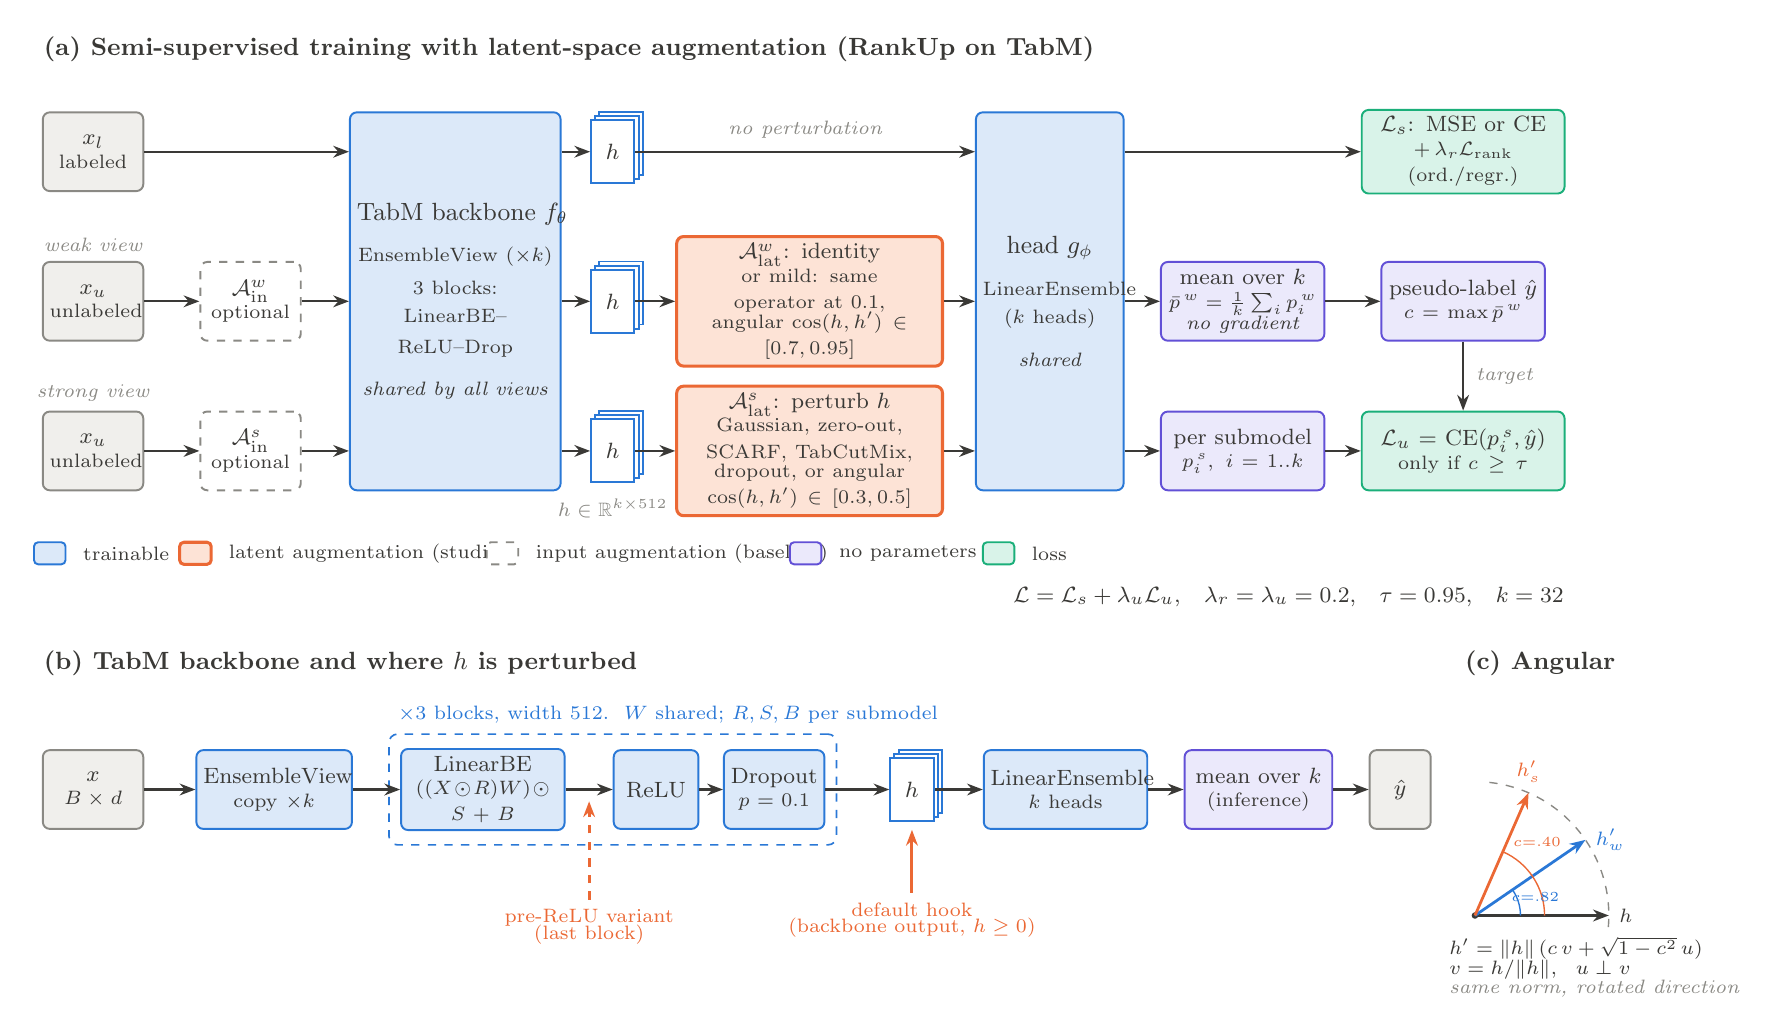
\begin{tikzpicture}

% ============================ (a) training pipeline ============================
\node[title] at (-0.75, 1.3) {(a) Semi-supervised training with latent-space augmentation (RankUp on TabM)};

\def\yL{0} \def\yW{-1.9} \def\yS{-3.8}

\node[data] (xl) at (0,\yL) {$x_l$\\[-1pt]{\scriptsize labeled}};
\node[data] (xw) at (0,\yW) {$x_u$\\[-1pt]{\scriptsize unlabeled}};
\node[data] (xs) at (0,\yS) {$x_u$\\[-1pt]{\scriptsize unlabeled}};
\node[note, above=0pt of xw] {weak view};
\node[note, above=0pt of xs] {strong view};

\node[inaug] (iw) at (2.0,\yW) {$\mathcal{A}^{w}_{\mathrm{in}}$\\[-1pt]{\scriptsize optional}};
\node[inaug] (is) at (2.0,\yS) {$\mathcal{A}^{s}_{\mathrm{in}}$\\[-1pt]{\scriptsize optional}};

\node[model, text width=25mm, minimum height=48mm] (bb) at (4.6,-1.9)
  {\small\mbox{TabM backbone $f_\theta$}\\[4pt]
   {\scriptsize\mbox{EnsembleView ($\times k$)}}\\[1pt]
   {\scriptsize 3 blocks:}\\[-1pt]{\scriptsize LinearBE--ReLU--Drop}\\[6pt]
   {\scriptsize\itshape shared by all views}};

\node[tensor] (hl) at (6.6,\yL) {$h$};
\node[tensor] (hw) at (6.6,\yW) {$h$};
\node[tensor] (hs) at (6.6,\yS) {$h$};
\node[note, below=2pt of hs] {$h\in\mathbb{R}^{k\times 512}$};

\node[lataug] (aw) at (9.1,\yW) {$\mathcal{A}^{w}_{\mathrm{lat}}$: identity\\[-1pt]{\scriptsize or mild: same operator at 0.1,}\\[-2.5pt]{\scriptsize angular $\cos(h,h')\in[0.7,0.95]$}};
\node[lataug] (as) at (9.1,\yS) {$\mathcal{A}^{s}_{\mathrm{lat}}$: perturb $h$\\[-1pt]
  {\scriptsize Gaussian, zero-out, SCARF, TabCutMix,}\\[-2.5pt]{\scriptsize dropout, or angular $\cos(h,h')\in[0.3,0.5]$}};

\node[model, text width=17mm, minimum height=48mm] (hd) at (12.15,-1.9)
  {\small head $g_\phi$\\[4pt]{\scriptsize LinearEnsemble}\\[-1pt]{\scriptsize ($k$ heads)}\\[6pt]{\scriptsize\itshape shared}};

\node[op] (mean) at (14.6,\yW) {mean over $k$\\[-1pt]{\scriptsize $\bar p^{\,w}=\frac{1}{k}\sum_i p^{\,w}_i$}\\[-2pt]{\scriptsize\itshape no gradient}};
\node[op] (pl)   at (17.4,\yW) {pseudo-label $\hat y$\\[-1pt]{\scriptsize $c=\max\bar p^{\,w}$}};
\node[op] (zs)   at (14.6,\yS) {per submodel\\[-1pt]{\scriptsize $p^{\,s}_i,\ i=1..k$}};
\node[loss] (lu) at (17.4,\yS) {$\mathcal{L}_u=\mathrm{CE}(p^{\,s}_i,\hat y)$\\[-1pt]{\scriptsize only if $c\ge\tau$}};
\node[loss] (ls) at (17.4,\yL) {$\mathcal{L}_s$: MSE or CE\\[-1pt]{\scriptsize $+\,\lambda_r\mathcal{L}_{\mathrm{rank}}$ (ord./regr.)}};

% labeled row
\draw[flow] (xl) -- (xl -| bb.west);
\draw[flow] (bb.east |- hl) -- (hl);
\draw[flow] (hl) -- node[note, above=1pt] {no perturbation} (hl -| hd.west);
\draw[flow] (hd.east |- ls) -- (ls);
% weak row
\draw[flow] (xw) -- (iw);
\draw[flow] (iw) -- (iw -| bb.west);
\draw[flow] (bb.east |- hw) -- (hw);
\draw[flow] (hw) -- (aw);
\draw[flow] (aw) -- (aw -| hd.west);
\draw[flow] (hd.east |- mean) -- (mean);
\draw[flow] (mean) -- (pl);
% strong row
\draw[flow] (xs) -- (is);
\draw[flow] (is) -- (is -| bb.west);
\draw[flow] (bb.east |- hs) -- (hs);
\draw[flow] (hs) -- (as);
\draw[flow] (as) -- (as -| hd.west);
\draw[flow] (hd.east |- zs) -- (zs);
\draw[flow] (zs) -- (lu);
\draw[flow] (pl) -- node[note, right=1pt] {target} (lu);

\node[anchor=east] at (18.8,-5.65)
  {$\mathcal{L}=\mathcal{L}_s+\lambda_u\mathcal{L}_u$,\quad $\lambda_r=\lambda_u=0.2$,\quad $\tau=0.95$,\quad $k=32$};

\begin{scope}[shift={(-0.55,-5.1)}]
  \node[key, fill=modelF, draw=modelE] at (0,0) {};
  \node[font=\scriptsize, anchor=west] at (0.3,0) {trainable};
  \node[key, fill=augF, draw=augE, line width=1.1pt] at (1.85,0) {};
  \node[font=\scriptsize, anchor=west] at (2.15,0) {latent augmentation (studied)};
  \node[key, fill=white, draw=muted, dashed] at (5.75,0) {};
  \node[font=\scriptsize, anchor=west] at (6.05,0) {input augmentation (baseline)};
  \node[key, fill=opF, draw=opE] at (9.6,0) {};
  \node[font=\scriptsize, anchor=west] at (9.9,0) {no parameters};
  \node[key, fill=lossF, draw=lossE] at (12.05,0) {};
  \node[font=\scriptsize, anchor=west] at (12.35,0) {loss};
\end{scope}

% ============================ (b) TabM and hook position ============================
\node[title] at (-0.75,-6.5) {(b) TabM backbone and where $h$ is perturbed};

\def\yB{-8.1}
\node[data] (bx) at (0,\yB) {$x$\\[-1pt]{\scriptsize $B\times d$}};
\node[model, text width=18mm] (ev) at (2.3,\yB) {EnsembleView\\[-1pt]{\scriptsize copy $\times k$}};
\node[model, text width=19mm] (lbe) at (4.95,\yB) {LinearBE\\[-1pt]{\scriptsize $((X\!\odot\! R)W)\!\odot\! S+B$}};
\node[model, text width=9mm] (relu) at (7.15,\yB) {ReLU};
\node[model, text width=11mm] (drop) at (8.65,\yB) {Dropout\\[-1pt]{\scriptsize $p=0.1$}};
\begin{scope}[on background layer]
  \node[draw=modelE, dashed, rounded corners=3pt, line width=0.6pt, fit=(lbe)(relu)(drop), inner xsep=4pt, inner ysep=5pt] (blk) {};
\end{scope}
\node[font=\scriptsize, text=modelE, anchor=south west, align=left] at (blk.north west)
  {$\times 3$ blocks, width 512.\ \ $W$ shared; $R,S,B$ per submodel};
\node[tensor] (bh) at (10.4,\yB) {$h$};
\node[model, text width=19mm] (lin) at (12.35,\yB) {LinearEnsemble\\[-1pt]{\scriptsize $k$ heads}};
\node[op, text width=17mm] (bmean) at (14.8,\yB) {mean over $k$\\[-1pt]{\scriptsize (inference)}};
\node[data, text width=6mm] (by) at (16.6,\yB) {$\hat y$};

\draw[flow] (bx) -- (ev);
\draw[flow] (ev) -- (lbe);
\draw[flow] (lbe) -- (relu);
\draw[flow] (relu) -- (drop);
\draw[flow] (drop) -- (bh);
\draw[flow] (bh) -- (lin);
\draw[flow] (lin) -- (bmean);
\draw[flow] (bmean) -- (by);

\coordinate (pre) at ($(lbe.east)!0.5!(relu.west)$);
\draw[augE, line width=1.1pt, -{Stealth[length=2mm]}] ($(bh.south)+(0,-0.9)$) -- ($(bh.south)+(0,-0.1)$);
\node[font=\scriptsize, text=augE, anchor=north] at ($(bh.south)+(0,-0.9)$) {default hook\\[-2pt](backbone output, $h\ge 0$)};
\draw[augE, line width=1.1pt, dashed, -{Stealth[length=2mm]}] ($(pre)+(0,-1.4)$) -- ($(pre)+(0,-0.15)$);
\node[font=\scriptsize, text=augE, anchor=north] at ($(pre)+(0,-1.4)$) {pre-ReLU variant\\[-2pt](last block)};

% ============================ (c) angular augmentation ============================
\node[title] at (17.3,-6.5) {(c) Angular};
\begin{scope}[shift={(17.55,-9.7)}, scale=1.7]
  \draw[muted, dashed, line width=0.5pt] (-5:1) arc (-5:85:1);
  \fill[ink] (0,0) circle (0.7pt);
  \draw[-{Stealth[length=2mm]}, line width=1pt, ink] (0,0) -- (0:1) node[right, font=\scriptsize] {$h$};
  \draw[-{Stealth[length=2mm]}, line width=1pt, modelE] (0,0) -- (34.4:1) node[right, font=\scriptsize, text=modelE] {$h'_w$};
  \draw[-{Stealth[length=2mm]}, line width=1pt, augE] (0,0) -- (66.4:1) node[above, font=\scriptsize, text=augE] {$h'_s$};
  \draw[modelE, line width=0.5pt] (0:0.34) arc (0:34.4:0.34);
  \draw[augE, line width=0.5pt] (0:0.52) arc (0:66.4:0.52);
  \node[font=\tiny, text=modelE] at (17:0.47) {$c$=.82};
  \node[font=\tiny, text=augE, fill=white, inner sep=0.5pt] at (50:0.72) {$c$=.40};
\end{scope}
\node[font=\scriptsize, anchor=north west, align=left] at (17.1,-9.85)
  {$h'=\|h\|\,(c\,v+\sqrt{1-c^2}\,u)$\\[-1pt]
   $v=h/\|h\|,\ \ u\perp v$\\[-1pt]
   {\itshape\color{muted} same norm, rotated direction}};

\end{tikzpicture}
\end{document}
